\documentclass[../notes.tex]{subfiles}

\pagestyle{main}
\renewcommand{\chaptermark}[1]{\markboth{\chaptername\ \thechapter\ (#1)}{}}
\setcounter{chapter}{2}

\begin{document}




\chapter{Electron Microscopy}
\section{Diamond Anvil Cell + Scanning Electron Microscopy}
\begin{itemize}
    \item \marginnote{1/17:}There will be a demonstration class with Dr. Filatov some afternoon. He will show us how to run some experiments, both sample-wise and data-wise.
    \item Review of DAC content from last class.
    \item Diamond anvil cell program and GSECARRs.
    \begin{itemize}
        \item UChicago's dedicated beamline is Sector 13.
        \item It pulls electrons out of the storage ring using IDs or BMs.
        \item "S" on this slide stands for single-crystal.
        \item DACs are now automated to a very large extent; no more manual screw adjustment.
    \end{itemize}
    \item An example experiment: Phase relations of iron carbides at high temperatures and pressures.
    \begin{itemize}
        \item You don't need to remember this; it's just to give you a flavor of what can be done.
        \item These compounds are applicable to geology since they're often far in the ground.
        \item DACs and laser heating replicate the heat and pressure present deep in the earth.
        \item The researchers built a phase diagram from the XRD spectra of both solid and liquid phases.
        \item Main takeaway: You can study more than crystalline phase transitions; indeed, even solid-to-liquid transitions are on the table.
    \end{itemize}
    \item Another example experiment: Magnesium peroxide formation.
    \begin{itemize}
        \item Magnesium peroxide is present in some geological objects.
        \item In these experiments, researchers recreated the conditions that can cause the geological formation of \ce{MgO2} over \ce{MgO} to observe how it happens.
    \end{itemize}
    \item One more example experiment: \ce{NaCl} stoichiometry
    \begin{itemize}
        \item Published in Science: You'd think it'd be hard to be surprised by a result about \ce{NaCl} at this point, but these scientists proved the existence of \ce{Na3Cl} and \ce{NaCl3} at high pressures.
        \item \ce{Na3Cl} is composed of layers of pure sodium and layers of \ce{NaCl}.
        \item These new "isomers" have special properties, e.g., the pure sodium layer in \ce{Na3Cl} conducts electricity in two-dimensions, and the surrounding \ce{NaCl} layers act as insulators.
        \item Good follow-up question: What is the charge? Could \ce{Na3Cl}, for instance, still be neutral?
        \item Shevchenko recommends we check out the paper: \textcite{bib:NaClStoichiometry}.
    \end{itemize}
    \item Challenges for DAC studies.
    \begin{itemize}
        \item Chemical reaction of sample/medium with diamond.
        \begin{itemize}
            \item Especially prevalent with alkali metals and hydrogen.
        \end{itemize}
        \item Any imperfections in the diamond anvil culet surface cause them to easily crack.
        \begin{itemize}
            \item Cracking the diamond forces you not just to get new diamonds (expensive), but to have to restart your experiment (costly in terms of time).
        \end{itemize}
        \item Hydrogen penetrates the metal gasket and diamond anvils easily at higher temperatures and pressures.
        \item Solution: Use cryogenic temperatures (just slow down the process).
        \begin{itemize}
            \item Even in this case, you can still do heating experiments; you just have to \emph{locally} heat your sample.
        \end{itemize}
    \end{itemize}
    \item Synthesis of new materials.
    \begin{itemize}
        \item Procedure: Synthesize a material, create possible models of it, calculate the predicted XRD pattern, test alignment with the actual XRD pattern.
        \item Example: \ce{NaH3} with elongated molecules of \ce{H2} incorporated into the crystal lattice.
    \end{itemize}
    \item First DAC experiments on nanomaterials.
    \begin{itemize}
        \item First conducted by Sarah H. Tolbert (now a UCLA prof) and A. P. Alivisatos in 1995.
        \item Examined pressure-induced structural transformations in semiconductor nanocrystals.
        \item Observed elevation in solid-solid structural transformation pressure as crystallite size decreases.
        \item Example: \ce{CdSe} nanocrystals.
        \begin{itemize}
            \item The \ce{CdSe} nanocrystals undergo a wurtzite to rock salt transition (similar to bulk \ce{CdSe}).
            \item The nanocrystal phase transition pressures varied from \SIrange{3.6}{4.9}{\giga\pascal} for crystallites ranging from \SIrange{21}{10}{\angstrom} in radius (bulk \ce{CdSe}: \SI{2.0}{\giga\pascal}).
            \item Demonstrated that the transition only nucleates once in each nanocrystal.
        \end{itemize}
    \end{itemize}
    \item Probing of mechanical properties using DAC.
    \begin{itemize}
        \item DACs are often used to probe nanoparticle assemblies.
        \item NPs can be assembled into periodic structures (recall the first class).
        \item Compress a ruby and \ce{PbS} up to \SI{50}{\giga\pascal}.
        \item Can you bring NPs close enough together to observe collective properties? At close enough distances, the organic strings around them intercalate. Can you push them even closer?
        \item The computer simulations of this took much longer than the actual DAC experiment.
        \item Removing pressure allows elastic recovery.
        \item Conclusions: In this case, we could not bring particles close enough together to observe collected properties. Not conclusive though; maybe other ligands, more pressure would work.
    \end{itemize}
    \item High-pressure structural stability and elasticity.
    \begin{itemize}
        \item Many cases of using DACs to study structures made out of gold or \ce{CoO} particles.
        \item Recall that NPs are often single crystals.
        \item NPs can have a preferred orientation when we compress them.
    \end{itemize}
    \item Mechanical stability of crystals assembled from \ce{Fe_xO_y} NPs.
    \begin{itemize}
        \item Vacant, polycrystalline shells should implode/explode upon isotropic compression, but instead they are very stable (maybe something to do with the spherical shape).
    \end{itemize}
    \item How "hollow" are hollow \ce{Fe_xO_y} NPs?
    \begin{itemize}
        \item Alivisatos is often mentioned in this course because he did actually play a very big role in the development of nanoscience.
        \item This example is from Shevchenko's own work.
        \item At high temperatures, NPs start to seed; you end up with large blobs. Thus, reactivity goes down (if you've got catalysts mounted on their surface).
        \item The shell is not penetrable to gases.
        \begin{itemize}
            \item Pores (defects) can allow gases to enter in theory, though.
        \end{itemize}
        \item Inside the shell, there are tiny fragment of \ce{Fe} or \ce{Fe_xO_y}.
        \item These particles are hoped to be able to deliver drugs since they have pores.
        \item If \ce{He} or \ce{Ne} diffuses into the NPs, we know that \ce{Ne} crystallizes upon compression, so if it goes into the NPs, then you start to see broader peaks (relation to Figure \ref{fig:strains}??).
        \begin{itemize}
            \item This was not observed, so Shevchenko concluded that \ce{Fe_xO_y} shells do not allow the transport of atoms in and out.
        \end{itemize}
    \end{itemize}
    \item Pressure-mediated doping in graphene.
    \begin{itemize}
        \item Alcohol was used as a pressure transmitting media.
        \item Raman spectroscopy monitored the transition in graphene.
        \item Conclusion: Alcohol can dope graphene upon compression.
        \item No doping is observed when \ce{Ar} is used as a pressure transmitting medium.
        \item First reported in 2011 (when graphene was exploding); mechanism in 2017.
        \item Conclusion: Electron charge injection is through the \ce{SiO2} substrate.
        \item The formation of silanol groups (\ce{Si-O-H}) on the surface of oxidized silicon substrates (similar to CNTs) --- origin of doping in graphene.
    \end{itemize}
    \item Pressure studies on MOFs.
    \begin{itemize}
        \item Since MOFs are promising for separation (which requires compression at some point), researchers wanted to know how they behave under compression.
        \item Different behavior under pressure? And can liquid get inside MOF shells under pressure?
        \item Pressure-transmitting medium 1 was \ce{NaCl}: Irreversible amorphization (collapsing) of the empty structure occurs at about \SI{0.4}{\giga\pascal}.
        \item Pressure-transmitting medium 2 was oil: Slight lattice expansion and a strong modification of the peak frequency and shape of the MOF hydroxyl vibration below \SI{0.1}{\giga\pascal}.
        \item Pressure-transmitting medium 3 was high-viscosity polydimethylsiloxane silicone oil: Framework stability is enhanced under pressure with the amorphization onset shifted to about \SI{7}{\giga\pascal}.
    \end{itemize}
    \item Why were the media from previous selected?
    \begin{figure}[h!]
        \centering
        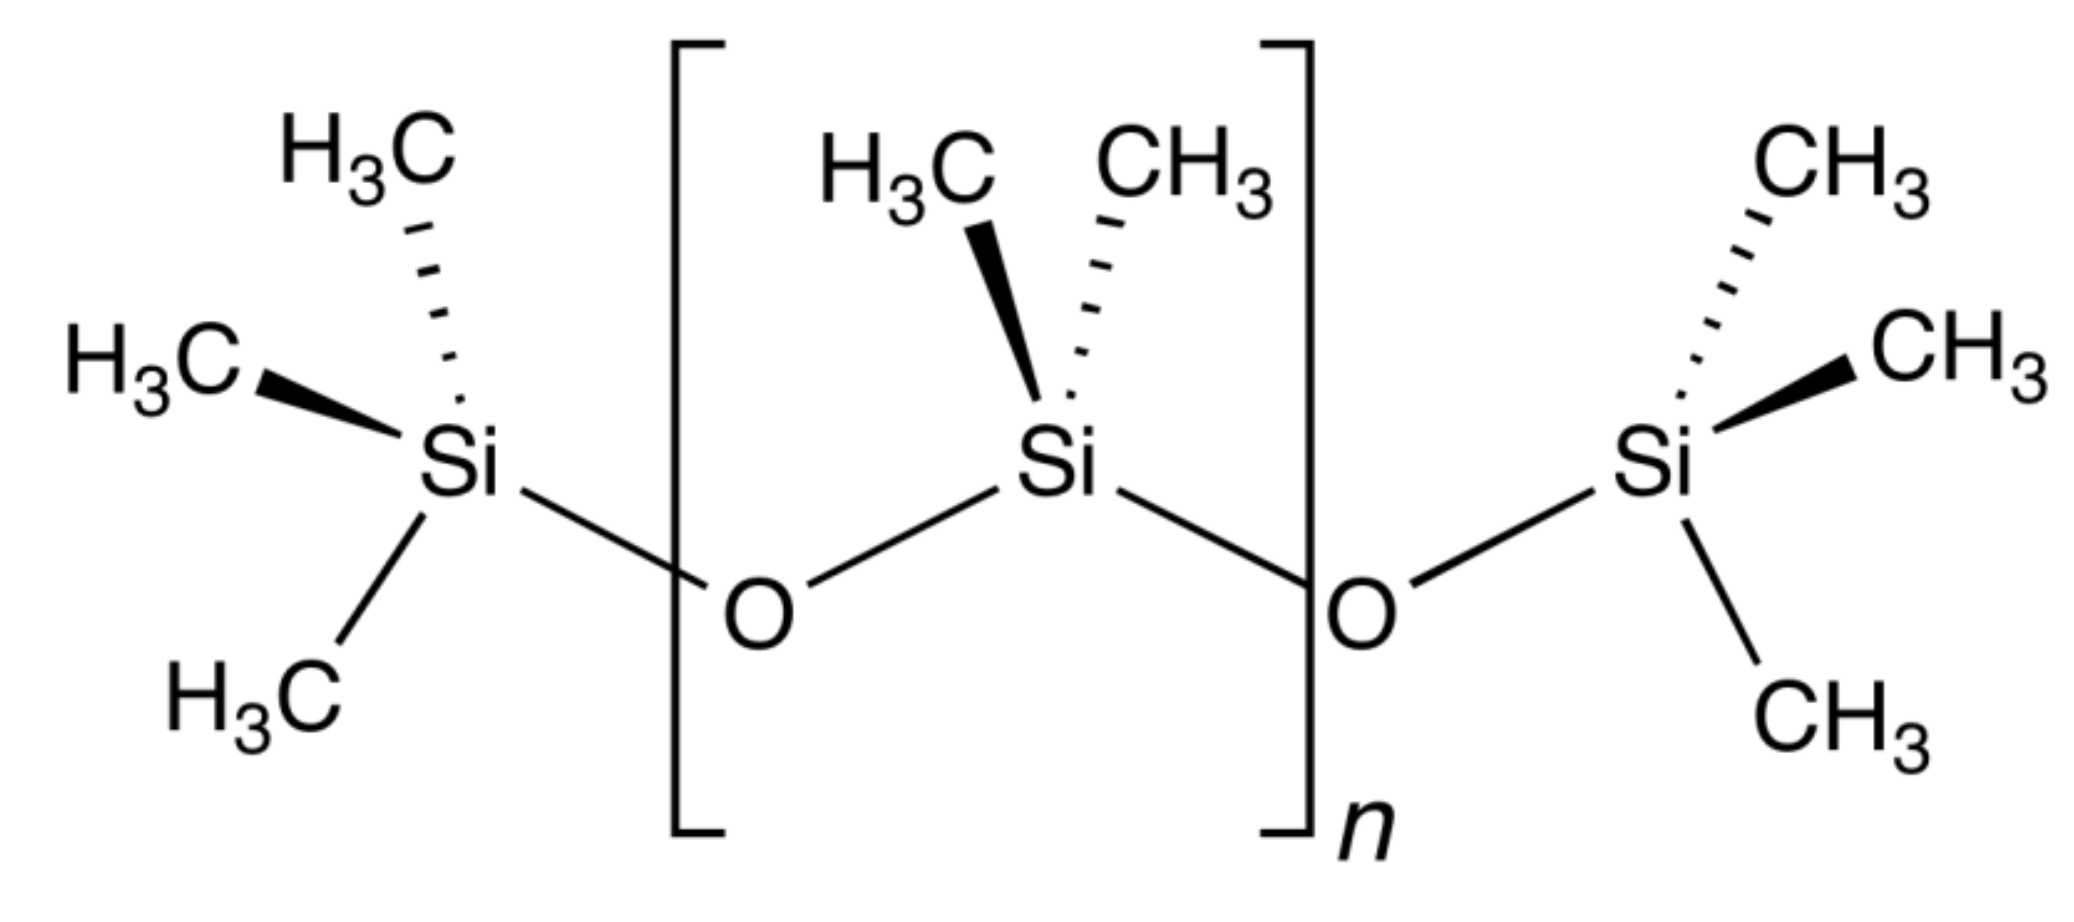
\includegraphics[width=0.35\linewidth]{PDMSSiliconeOil.png}
        \caption{Polydimethylsiloxane silicone oil.}
        \label{fig:PDMSSiliconeOil}
    \end{figure}
    \begin{itemize}
        \item \ce{NaCl}: Optically transparent in the study areas, so minimal background interference.
        \item Nujol: An inert mineral oil used in infrared spectroscopy. It has a relatively simple IR spectrum.
        \item Polydimethylsiloxane silicone oil: Inert and optically transparent.
        \item You have to be sure that your medium does not overlap with your sample.
    \end{itemize}
    \item Pressure-mediated changes in MOFs.
    \begin{figure}[h!]
        \centering
        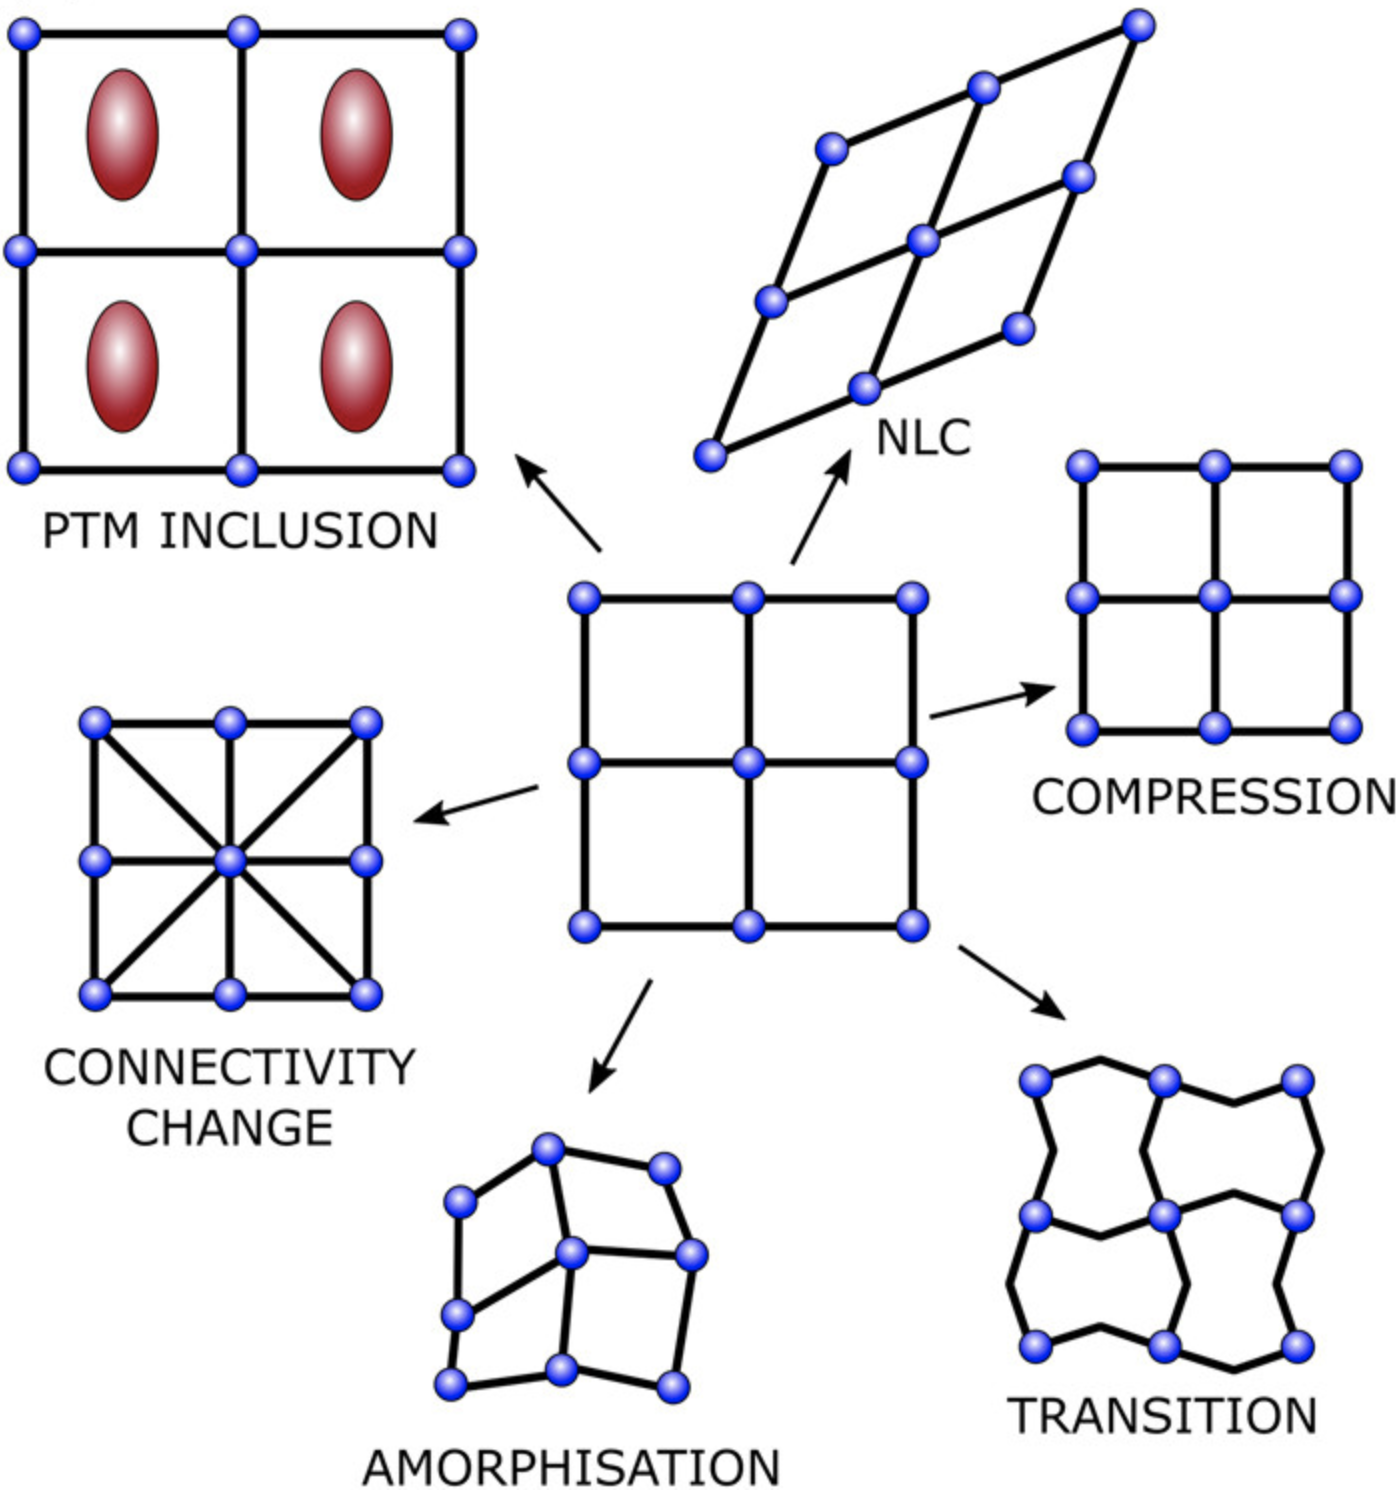
\includegraphics[width=0.4\linewidth]{MOFPressure.png}
        \caption{MOFs under extreme pressure.}
        \label{fig:MOFPressure}
    \end{figure}
    \begin{itemize}
        \item Negative linear compressibility (NLC).
        \begin{itemize}
            \item Either causes expansion or net zero compressibility (compressibility along one or two axes, expansion along two or one).
        \end{itemize}
        \item Compression.
        \item Transition.
        \item Amorphisation.
        \begin{itemize}
            \item Note that transition preserves crystallinity in some form, while amorphisation does away with it entirely.
        \end{itemize}
        \item Connectivity change.
        \item Pressure-transmitting medium (PTM) inclusion.
    \end{itemize}
    \item Summary of DAC studies.
    \begin{itemize}
        \item Use them to\dots
        \begin{itemize}
            \item Study phase transformation;
            \item Study the synthesis of novel materials;
            \item Understand the universe/the formation of extant Earthbound or extraterrestrial minerals.
        \end{itemize}
    \end{itemize}
    \item We now move on to scanning electron microscopy.
    \item Examples of SEM images.
    \begin{itemize}
        \item Pollen from different plants, the eye of a fruit fly, and opal.
        \begin{itemize}
            \item Note that opal is made of (possible fused) silicon beads of either uniform or different sizes.
        \end{itemize}
        \item False color: Allows you to highlight certain features.
    \end{itemize}
    \item First SEM.
    \begin{itemize}
        \item The concepts was first proposed in 1935 by Max Knoll.
        \item At the time, researchers were actively working on using electrons for imaging but were focusing on transmission.
        \item Manfred von Ardenne designed the first scanning transmission electron microscope (STEM) in 1937-38 by adding scan coils to a transmission electron microscope to surpass its resolution.
        \item The first STEM microgaraph depicts \ce{ZnO} crystals imaged at an operating voltage of \SI{23}{\kilo\volt} at a magnification of \num{8000} times, and a spatial resolution between \SIrange{50}{100}{\nano\meter}.
        \begin{itemize}
            \item Nowadays, the resolution is about \SI{1.5}{\nano\meter}.
        \end{itemize}
        \item Keep in mind that SEM and STEM are different.
    \end{itemize}
    \item Interactions of electrons with matter.
    \begin{figure}[h!]
        \centering
        \begin{tikzpicture}
            \small
            \fill [gray!30] (-4,-0.3) rectangle (4,0.3);
            \node [right] at (4,0) {Thin sample};
    
            \footnotesize
            \draw [thick,-latex] (0,4) node[above]{Incident electrons} -- (0,0.3);
    
            \draw [semithick,-latex] (0,0.3) -- (1,3) node[above right,align=left]{Backscattered electrons\\{\color{blx}Atomic number and phase difference}};
            \draw [semithick,-latex] (0,0.3) -- (1.5,2) node[above right,align=left]{Bremsstrahlung radiation};
            \draw [semithick,-latex] (0,0.3) -- (2,1) node[above right,yshift=-2mm,align=left]{Secondary electrons\\{\color{blx}Topographic information}};
    
            \draw [semithick,-latex] (0,0.3) -- (-1,2.8) node[above left,align=left]{Visible light\\(cathodoluminescence)\\{\color{blx}Electronic states information}};
            \draw [semithick,-latex] (0,0.3) -- (-1.5,1.8) node[above left,align=left]{X-rays (EDS)\\{\color{blx}Thickness atomic composition}};
            \draw [semithick,-latex] (0,0.3) -- (-2,0.8) node[above left,yshift=-2mm,align=left]{Auger electrons\\{\color{blx}Surface atomic composition}};
    
            \draw [semithick,-latex] (0,-0.3) -- (1.2,-1.5) node[below right,align=left]{Elastically scattered electrons\\{\color{blx}Structural analysis (diffraction)}\\{\color{blx}and high-resolution imaging}};
            \draw [semithick,-latex] (0,-0.3) -- (0,-3) node[below,align=left]{Unscattered electrons\\{\color{blx}Morphological information}};
            \draw [semithick,-latex] (0,-0.3) -- (-1,-1.7) node[below left,align=left]{Inelastically scattered electrons\\{\color{blx}Composition and bond states (EELS)}\\{\color{blx}Z-contrast imaging HAADF}};
    
            \path (-6.5,0) -- (6.5,0);
        \end{tikzpicture}
        \caption{Interaction of electrons with matter.}
        \label{fig:ElectronsMatter}
    \end{figure}
    \begin{itemize}
        \item Consider a thin sample.
        \item We can cause a whole bunch of changes in our material with incoming electrons.
        \item We will talk about all of these eventually.
        \item SEM uses \textbf{backscattered electrons} and \textbf{secondary electrons}.
    \end{itemize}
    \item \textbf{Secondary electron}: An electron knocked out of a substance by a separate incident electron. \emph{Also known as} \textbf{SE}.
    \item \textbf{Backscattered electron}: An incident electron that gets rerouted back in the original direction via a close encounter with the nucleus. \emph{Also known as} \textbf{BSE}.
    \begin{itemize}
        \item Think "gravitational assist" from rocketry.
    \end{itemize}
    \item Bohr atomic model.
    \begin{itemize}
        \item Very simplistic, but says what we need. Shevchenko reviews Figure \ref{fig:bohrModel}.
        \item Generation of characteristic X-rays, depth profiles, and other phenomena.
    \end{itemize}
    \item Electron interaction volume within a sample.
    \begin{figure}[H]
        \centering
        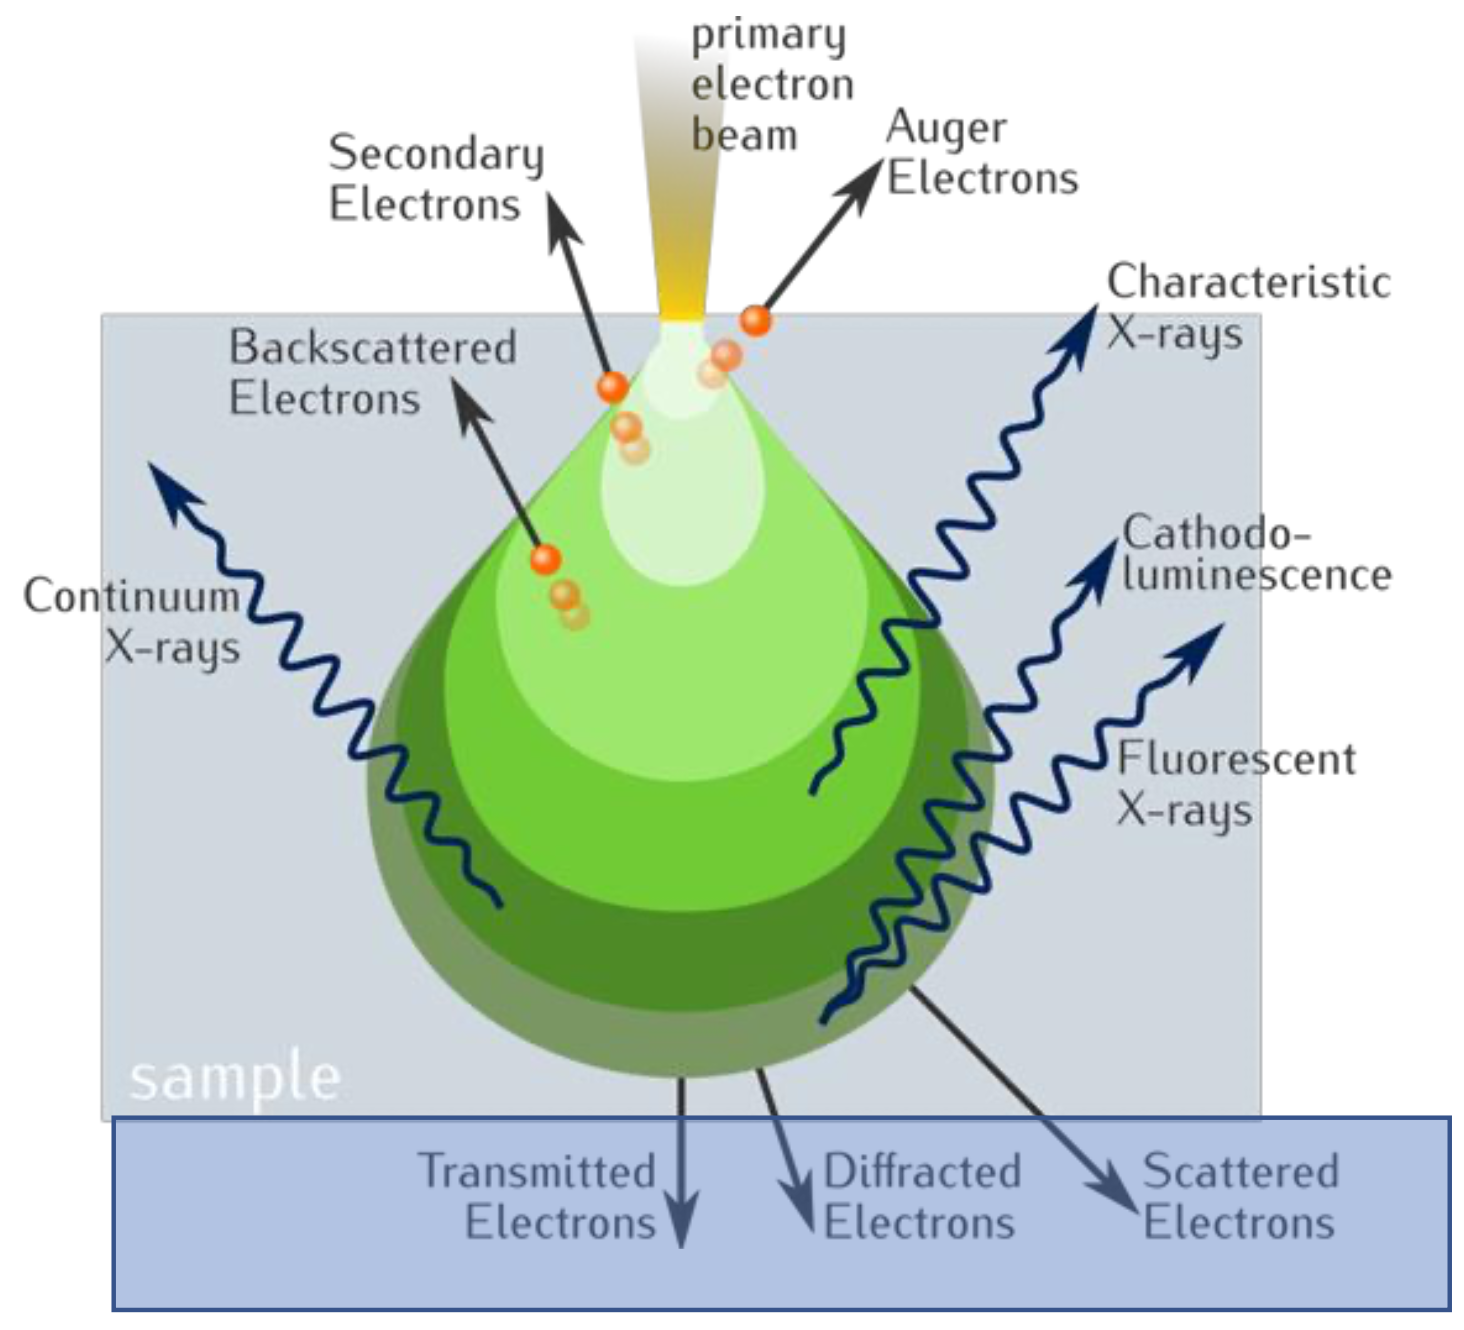
\includegraphics[width=0.4\linewidth]{eInteractionVolume.png}
        \caption{Electron interaction volume within a sample.}
        \label{fig:eInteractionVolume}
    \end{figure}
    \begin{itemize}
        \item \textbf{Auger electrons} are only generated at the very very top of the sample.
        \item The beam electron may be scattered inelastically by the Coulomb field of an atomic nucleus, losing some of its energy in the process as Bremsstrahlung radiation.
        \item The beam electrons can give up any amount of energy, so the energy distribution of the emitted X-rays is continuous up to the beam energy.
    \end{itemize}
    \item \textbf{Auger electron}: An electron that escapes its atom via the following process. \emph{Also known as} \textbf{AE}.
    \begin{enumerate}
        \item Incident electrons heat the atom.
        \item A core electron gets removed.
        \item A higher energy electron falls down, releasing energy as it does so.
        \item This energy is not released in the form of light, but is transferred to the electron of interest and used to escape.
    \end{enumerate}
    \item Example: Nickel.
    \begin{itemize}
        \item Conditions.
        \begin{itemize}
            \item Sample is predominantly $Z=28$.
            \item Accelerating voltage is \SI{20}{\kilo\volt}.
            \item \ang{0} tilt, i.e., incident beam is normal to specimen surface.
        \end{itemize}
        \item Penetrations.
        \begin{itemize}
            \item Augers: Only \SIrange{10}{30}{\angstrom}.
            \item Secondaries: Up to \SI{100}{\angstrom}.
            \item Backscattered: $<\SIrange{1}{2}{\micro\meter}$.
            \item Range of electron penetration: About \SI{5}{\micro\meter} in total.
        \end{itemize}
    \end{itemize}
    \item Secondary electrons.
    \begin{itemize}
        \item Often perform the SEM imaging.
        \item The electrons, once ionized, often leave the atom with a very small kinetic energy ($\sim\SI{5}{\electronvolt}$).
        \item There is only a slight energy loss and trajectory change in the incident electron; thus, each incident electron can produce several secondary electrons.
        \item Collection of these electrons is aided by using a \textbf{collector} in conjunction with the SE detector.
    \end{itemize}
    \item \textbf{Collector}: A grid or mesh with a \SI{+100}{\volt} potential applied to it which is placed in front of the detector, attracting the negatively charged secondary electrons to it which then pass through the grid holes and into the detector to be counted.
    \item Secondary electrons for imaging.
    \begin{itemize}
        \item Mostly effective up to \SI{5}{\nano\meter} in the material.
        \item Indeed, secondary electrons provide \textbf{surface topology imaging}.
        \begin{itemize}
            \item Due to their low energy, only SEs that are close to the surface can exit the sample.
            \item This small distance enables fine resolution in the SEM.
        \end{itemize}
        \item However, secondary electrons provide little-to-no information about elemental contribution.
        \item How does a detector tell electrons from the sample vs. the beam?
        \begin{itemize}
            \item We arrange the detector so that it only picks up electrons from one specific direction, and we control the direction to choose only electrons that are coming up at a particular angle.
        \end{itemize}
        \item Lighter elements have greater penetration depths.
        \item Secondary electrons are basically ionized electrons.
    \end{itemize}
    \item Imaging with secondary electrons.
    \begin{itemize}
        \item Extremely popular with nanofabrication.
    \end{itemize}
    \item Backscattered electrons (BSE).
    \begin{itemize}
        \item Elastic scattering happens with little loss of energy.
        \item BSEs provide elemental information since the number of BSEs produced is proportional to the atomic number of the elements within the specimen.
        \begin{itemize}
            \item Higher-atomic number elements "produce" more backscattered electrons and appear brighter than lower atomic number elements.
            \item This interaction is utilized to differentiate parts of the specimen that have different average atomic number.
        \end{itemize}
        \item Very popular for imaging metal alloys.
    \end{itemize}
    \item Imaging with backscattered electrons.
    \begin{itemize}
        \item We don't know flat vs. texture, but we can still see contrast in the images.
        \item In the picture in the slides, we can make out pores, as well as differentiate \ce{Mo}-rich (lighter colored) regions from \ce{Si}-rich (darker colored) regions.
        \begin{itemize}
            \item Since \ce{Mo} is higher-$Z$ than \ce{Si}, it makes sense that it should be lighter.
        \end{itemize}
    \end{itemize}
    \item Backscattered electrons vs. secondary electrons.
    \begin{itemize}
        \item Comparison of images for different alloys.
        \item SEs provide more information on the topology of the material.
        \begin{itemize}
            \item This information \emph{can} coincide with elemental information, but it does not have to.
        \end{itemize}
    \end{itemize}
    \item Characteristic X-rays.
    \begin{itemize}
        \item Utilized for elemental analysis since they're \emph{characteristic}.
        \item We have already discussed how these are generated.
        \item When electrons are not from the inner shell, an electron drops down, releasing energy in the form of photons in the process.
        \item Not relevant to SEM imaging; just elemental analysis.
    \end{itemize}
    \item Analytical use of characteristic X-rays.
    \begin{itemize}
        \item EDS=EDX: Energy dispersive spectroscopy and energy dispersive X-ray.
        \item Qualitative and quantitative analysis.
        \item EDS systems: X-ray detector plus software to collect and analyze energy spectra.
        \begin{itemize}
            \item Use \ce{Si}-\ce{Li} detectors, aka "silicon drift" detectors.
            \item Sometimes, such detectors need cooling systems. These are annoying to deal with, and thus are not present in more expensive models that use better, more idealized materials instead.
        \end{itemize}
        \item Working principle of the detector: The X-ray absorption converts the energy of individual X-rays into electrical voltages of proportional size.
        \begin{itemize}
            \item Incoming photons ionize the detector material, yielding free electrons in the crystal.
            \item The crystal becomes conductive and produces an electrical charge bias.
            \item The electrical pulses correspond to the characteristic X-rays of the element.
        \end{itemize}
    \end{itemize}
    \item Chemical information (EDS).
    \begin{itemize}
        \item Spectra, elemental mapping, and line scans.
    \end{itemize}
    \item Bremsstrahlung.
    \begin{itemize}
        \item Review of Figures \ref{fig:xrayTubeSpectrum}-\ref{fig:generationBremsstrahlung}.
    \end{itemize}
    \item Auger electrons (AE).
    \begin{itemize}
        \item Auger spectroscopy (AES) is liked by some researchers and is rapidly evolving right now.
        \begin{itemize}
            \item Carries information about the surface of the specimen (the first few atomic layers).
        \end{itemize}
        \item Since orbital energies are unique to an atom of a specific element, ejected electrons carry specific chemical information about the surface.
    \end{itemize}
    \item Building blocks of SEM.
    \begin{itemize}
        \item Electron source.
        \item Limiting apertures surround\dots
        \item Condenser lenses 1-2.
        \begin{itemize}
            \item These lenses focus them on a spot.
        \end{itemize}
        \item Then scanning coils.
        \item Lastly, an objective lens focuses everything downward.
        \item Three detectors.
        \begin{itemize}
            \item The BSE detector: A ring surrounding the point at which the incident electrons enter.
            \item The SE detector.
            \item The EDS detector.
        \end{itemize}
        \item These machines are big.
        \item The BSE detector is positioned as such so that it can catch backscattered electrons that circle around the nucleus and return close to their original trajectory.
        \item The apparatus doesn't move, but the beam does.
        \item The detectors stay where they are; you just change the beam position.
        \item By varying the current passing through the coils with the time, the position of the beam can be shifted (rastered).
        \item Many elements are similar to those in CTEM, but SEM images are not obtained all at once; rather, they are created in a rastering mode.
    \end{itemize}
    \item SEM resolution.
    \begin{itemize}
        \item High-Z materials have less penetration.
        \item More KE leads to a deeper penetration.
        \item Condenser lenses (1-2) focus the beam to a spot of $\sim\SIrange{0.4}{5}{\nano\meter}$, and they determine the focus of the instrument.
        \item Resolution can be limited by the interactions of electrons and materials.
        \begin{itemize}
            \item Dirty samples deposit carbon inside the instrument, spoiling the vacuum and harming the machine.
            \item Always be careful! Dirty samples are the product of lazy scientists.
        \end{itemize}
        \item Interaction volume depends on material: High-$Z$ materials have smaller interaction volumes.
        \item Interaction volume also depends on voltage.
        \begin{itemize}
            \item More voltage means a higher depth profile (may not be a good thing; for topology, you only want to study only the top surface).
        \end{itemize}
    \end{itemize}
    \item Astigmation of your images.
    \begin{itemize}
        \item Takes place when a lens field is not symmetrical in strength (weaker in one place than in another).
        \item Origins of astigmation.
        \begin{itemize}
            \item Imperfect polepiece boring.
            \item Nonhomogeneous blending of polepiece materials.
            \item Dirt on the polepieces, apertures, and/or specimen holders (most common).
        \end{itemize}
        \item Solution: A stigmator can be used to selectively correct the field.
        \begin{itemize}
            \item Stigmators produce weak fields compared to the electromagnetic lenses they correct.
        \end{itemize}
    \end{itemize}
    \item Detection of astigmation.
    \begin{itemize}
        \item Underfocusing the objective lens: Image details line up with the beam shape at that focus.
        \item Overfocusing: Image details line up along a direction orthogonal to the underfocused image.
        \item At exact focus: Image is OK-ish, but not really as sharp as it could be because the probe size (e.g., condensor) is larger than it should be.
        \item Essentially, turn the nob different ways until you get exact focus.
    \end{itemize}
    \item The last slide on astigmation.
    \begin{figure}[H]
        \centering
        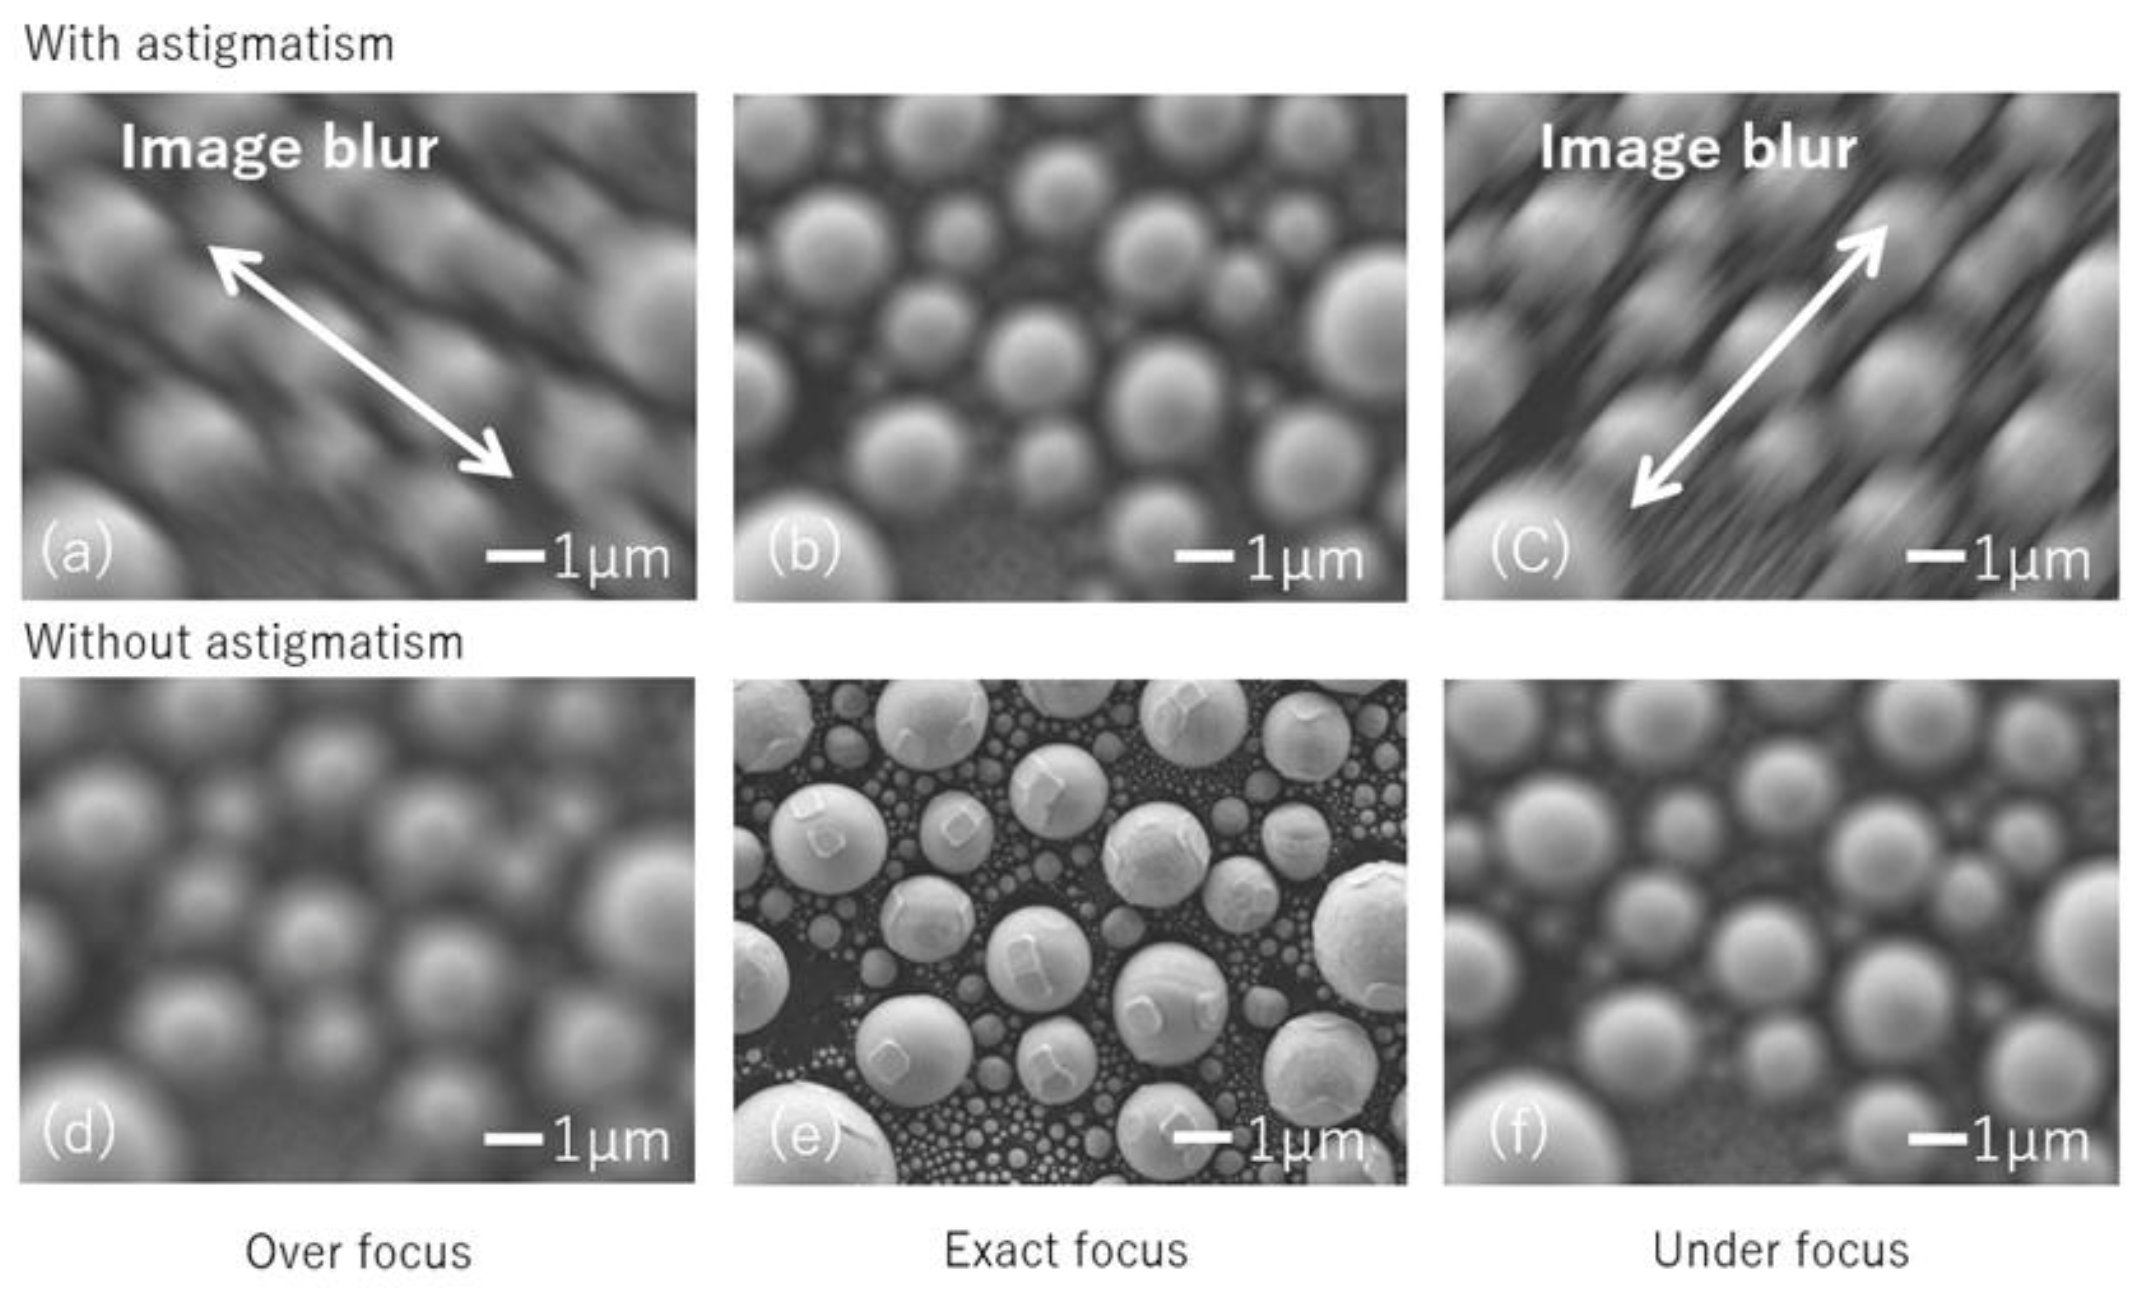
\includegraphics[width=0.65\linewidth]{astigmation.png}
        \caption{Correcting astigmation.}
        \label{fig:astigmation}
    \end{figure}
    \begin{itemize}
        \item It is really important to have good focus.
    \end{itemize}
\end{itemize}



\section{Scanning and Transmission Electron Microscopy}
\begin{itemize}
    \item \marginnote{1/19:}Image focusing.
    \begin{figure}[h!]
        \centering
        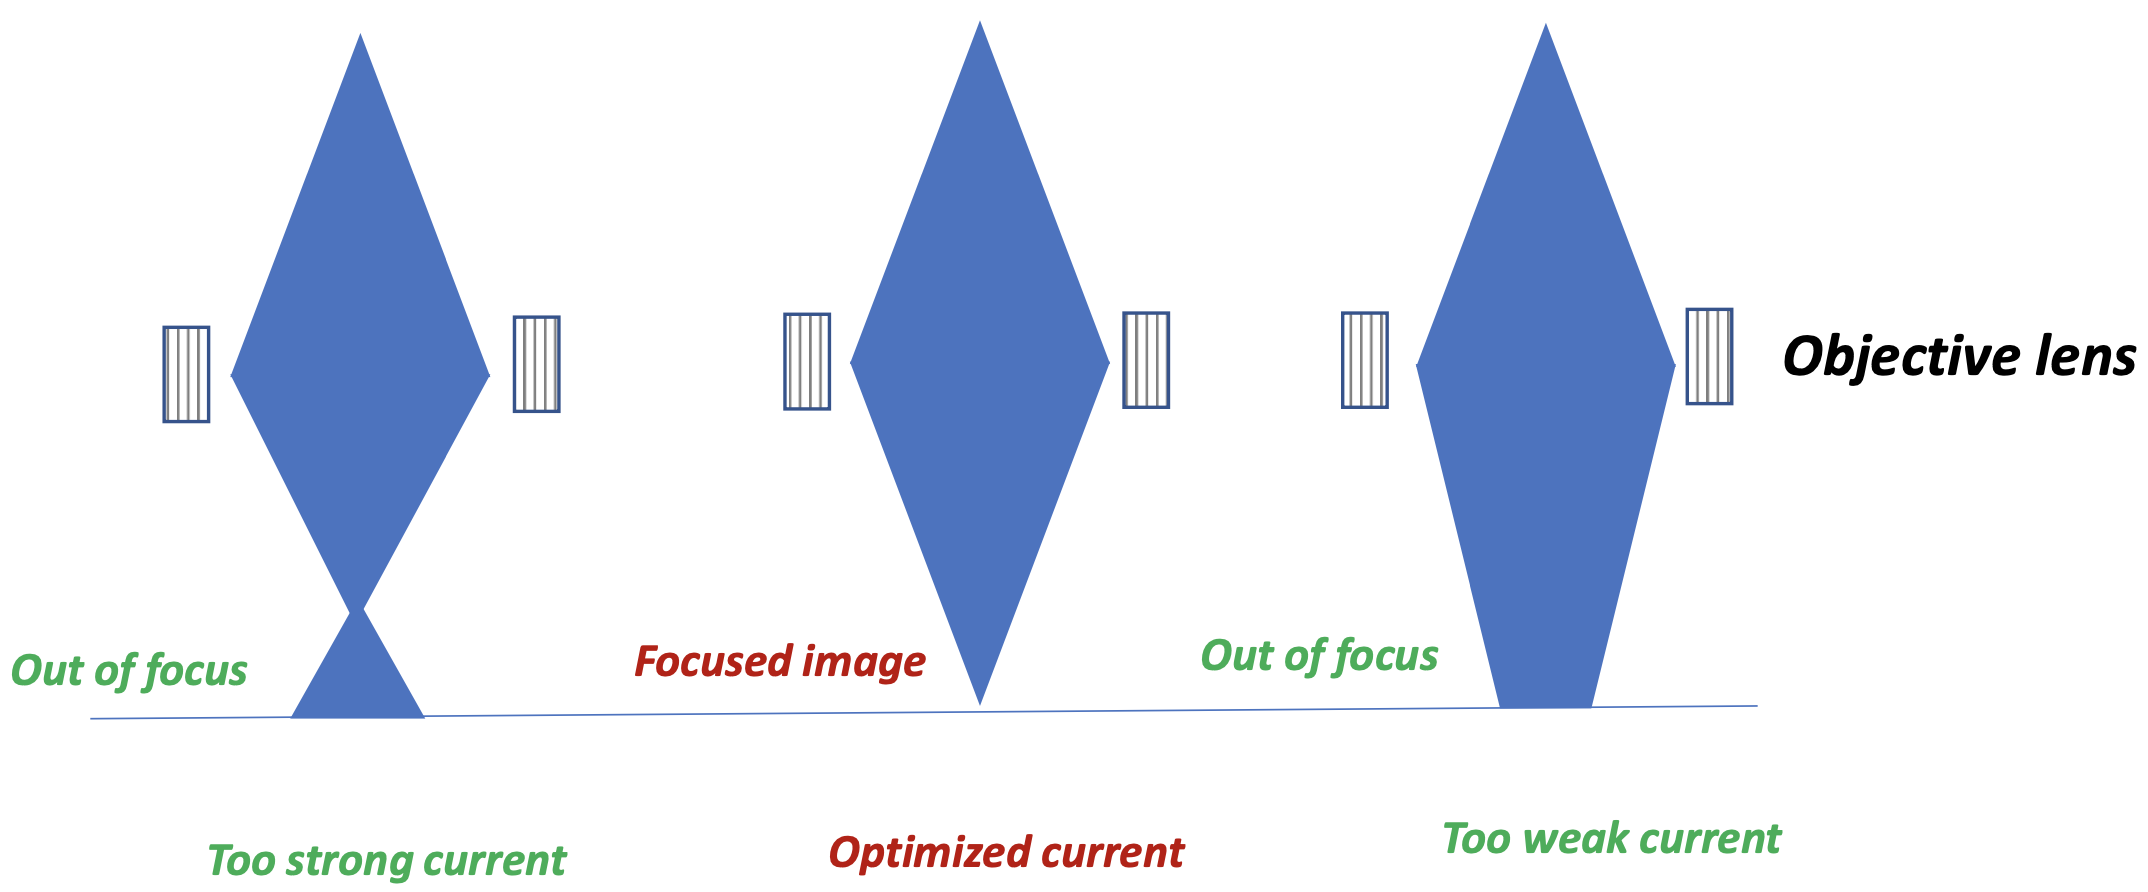
\includegraphics[width=0.75\linewidth]{imageFocusing.png}
        \caption{Image focusing.}
        \label{fig:imageFocusing}
    \end{figure}
    \begin{itemize}
        \item In optical microscopy, the focus is adjusted by moving the sample up and down.
        \item In SEM, we "move" the beam.
        \item In particular, we can adjust the magnetic field strength (and hence the focal length) of the OL by changing the current in it.
    \end{itemize}
    \item SEM vs. TEM.
    \begin{itemize}
        \item Example SEM vs. TEM images.
    \end{itemize}
    \item Design of the SEM instruments.
    \begin{itemize}
        \item Front-loading systems and sample transferring protocol.
    \end{itemize}
    \item Low vacuum SEM.
    \begin{itemize}
        \item Examples: Tabletop microscopes, environmental SEM.
        \item The pressure can be adjusted in the sample chamber until the "electron charging" is removed from images.
        \item Images without conductive coatings have lower resolutions.
        \item Example problem you can address with LV-SEM: Whether face masks are effective in preventing the spread of COVID-19.
        \begin{itemize}
            \item A \SI{1}{\micro\meter} polymer was used to mimic the virus.
        \end{itemize}
    \end{itemize}
    \item \textbf{Cryo-SEM}: A special method using a deep-cooled stage that allows imaging of \emph{hydrated} specimens by freezing the samples to very low temperatures (below \SI{-100}{\celsius}) where solid water is stable even in vacuum.
    \begin{itemize}
        \item Examples: Pictures of termites and collagen fibers.
    \end{itemize}
    \item Is it possible to do imaging using SEM?
    \begin{itemize}
        \item Yes??
    \end{itemize}
    \item Review of Figure \ref{fig:eInteractionVolume}.
    \begin{itemize}
        \item What was said here??
    \end{itemize}
    \item We now move onto transmission electron microscopy (TEM).
    \item Early TEM.
    \begin{itemize}
        \item In 1964, Dr. June Almeda took the first image of a coronavirus.
        \begin{itemize}
            \item Dr. Almeda attempted to report particles like this before while investigating infectious bronchitis in chickens.
            \item However, her paper was rejected because the reviewers said that the images could just be bad pictures of influenza virus particles.
        \end{itemize}
        \item More bio background on the development of TEM.
    \end{itemize}
    \item Size comparison.
    \begin{itemize}
        \item Light microscopes can resolve down to about \SI{100}{\nano\meter} (about the size of the flu virus).
        \item Electron microscopes can resolve from \SI{1}{\micro\meter} (about the size of a bacterium) down to about \SI{0.5}{\nano\meter} (about the size of a buckyball).
        \item Picture with more examples of objects in these size ranges.
    \end{itemize}
    \item Discovery of electrons.
    \begin{itemize}
        \item William Crookes of Crookes tubes returns!
        \item In 1879, he found that \textbf{cathode rays} can be bent by a magnetic field and the direction of the deflection indicated that there were negatively charged particles (different metals or gases inside??).
        \begin{itemize}
            \item However, these experiments did not settle the question of whether cathode rays were particles or radiation similar to light.
        \end{itemize}
        \item J. J. Thomson (1897): Studies cathode rays (in Crookes tubes with a good vacuum) between two parallel aluminum plates.
        \begin{itemize}
            \item If the top \ce{Al} electrode was negative, the rays moved down.
            \item If the top \ce{Al} electrode was positve, the rays moved up.
            \item Furthermore, the deflection was proportional to the difference in potential between the plates.
        \end{itemize}
        \item These two sets of experiments established that cathode rays could be deflected, and that this deflection behavior could be induced by magnetic and electric fields.
        \item Conclusion: Cathode rays have negatively charged particles (electrons).
        \item Impact:
        \begin{itemize}
            \item Shed light on the nature of electricity.
            \item Determined the ratio of mass-to-charge for the electron (very small, explaining why electrons can "flow" through metals).
        \end{itemize}
    \end{itemize}
    \item Charge of the electron.
    \begin{figure}[H]
        \centering
        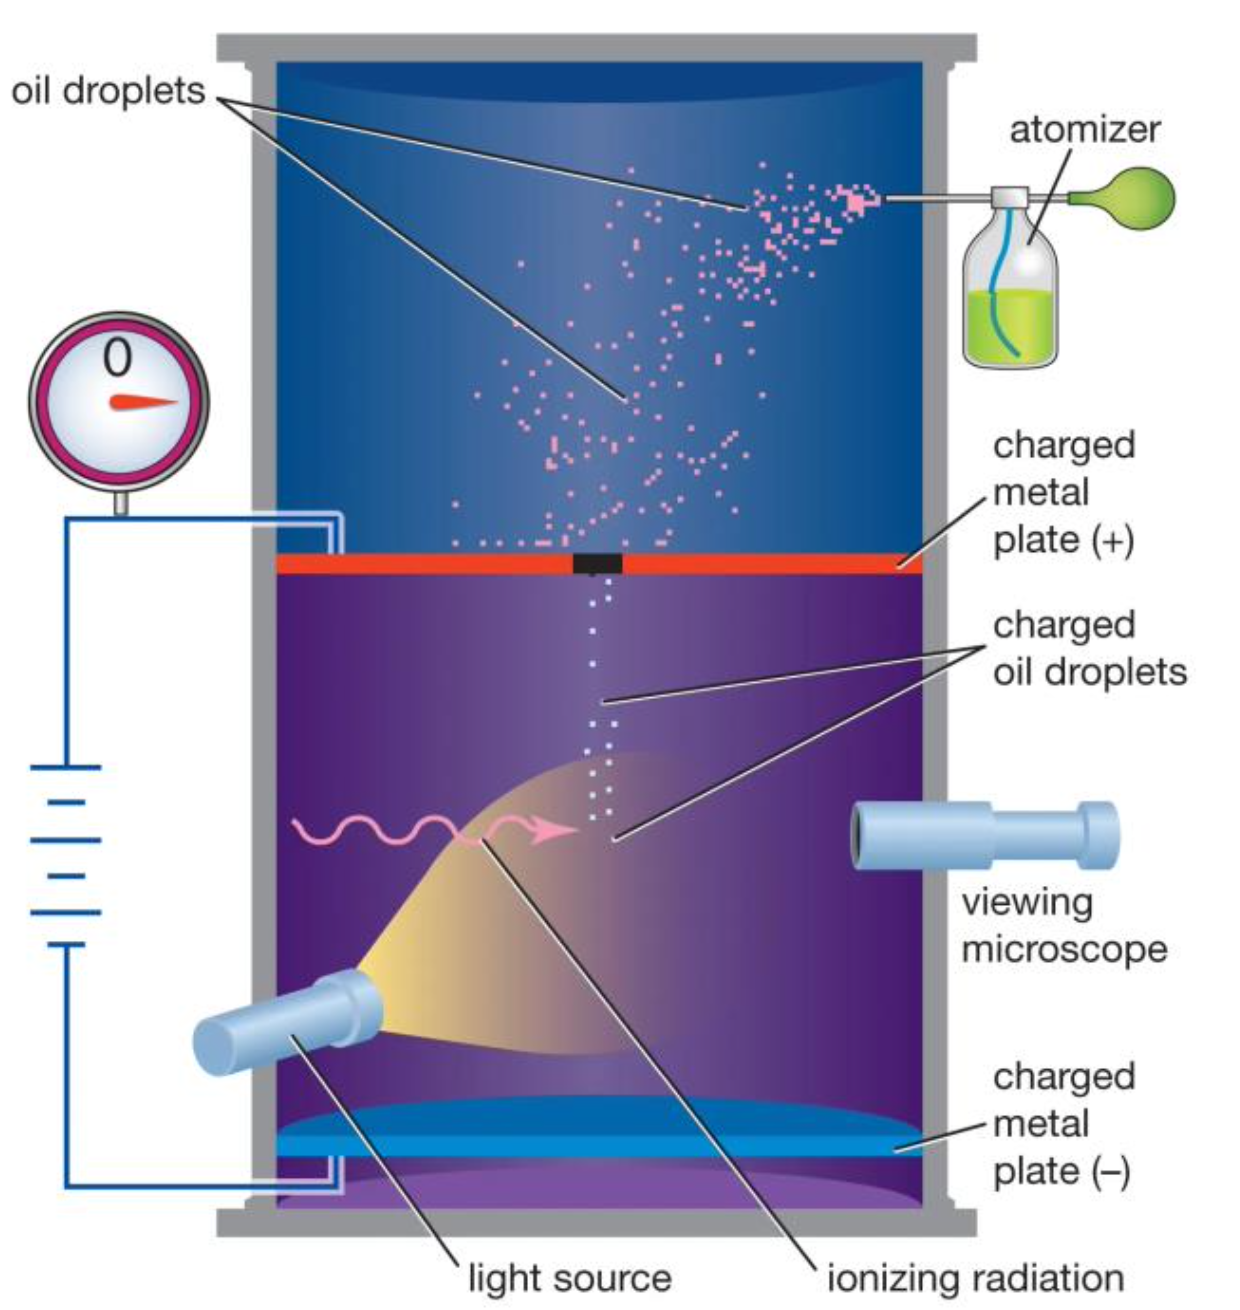
\includegraphics[width=0.3\linewidth]{oilDropExp.png}
        \caption{Oil-drop experiment.}
        \label{fig:oilDropExp}
    \end{figure}
    \begin{itemize}
        \item Robert Millikan (1910 at UChicago): Oil-drop experiment.
        \item X-rays interact with the oil and produce (a) charge(s) that is/are confined within a droplet.
        \item No charge applied: The fall of the droplet is determined by its mass and the medium's viscosity.
        \item Charge applied: The droplets stopped falling or even rose (depending on the number of charges).
        \item The position of droplets was dependent on the applied voltage.
        \item Millikan measured the electronic charge to two sig figs: \SI{1.6e-19}{\coulomb}.
    \end{itemize}
    \item Electrons as waves.
    \begin{itemize}
        \item Louis de Broglie (1924): Particles, such as electrons, could be described not only as particles but also as waves.
        \item Derivation of the de Broglie wavelength $\lambda_B$:
        \begin{equation*}
            \lambda_B = \frac{h}{p}
        \end{equation*}
        \item Photons always move at the same velocity (the speed of light).
        \item Particles, on the other hand, have mass and momentum. If $v\ll c$, then
        \begin{equation*}
            \lambda_B = \frac{h}{mv}
        \end{equation*}
        \item Keep in mind the difference between speed and velocity.
    \end{itemize}
    \item Early days of TEM.
    \begin{itemize}
        \item Max Knoll and Ernst Ruska (1931): The first transmission microscope.
        \begin{itemize}
            \item Ruska won the 1986 Nobel prize in physics for his many achievements in electron optics.
        \end{itemize}
        \item 1939: First commercial TEM.
        \item Working principle of TEM.
        \begin{itemize}
            \item Similar to that of light microscopes: Light rays used to focus and produce an image vs. a beam of electrons used to focus on the sample to produce an image.
            \item Electrons have much shorter wavelengths than light.
        \end{itemize}
    \end{itemize}
    \item Building blocks of the TEM.
    \begin{figure}[H]
        \centering
        \begin{subfigure}[b]{0.4\linewidth}
            \centering
            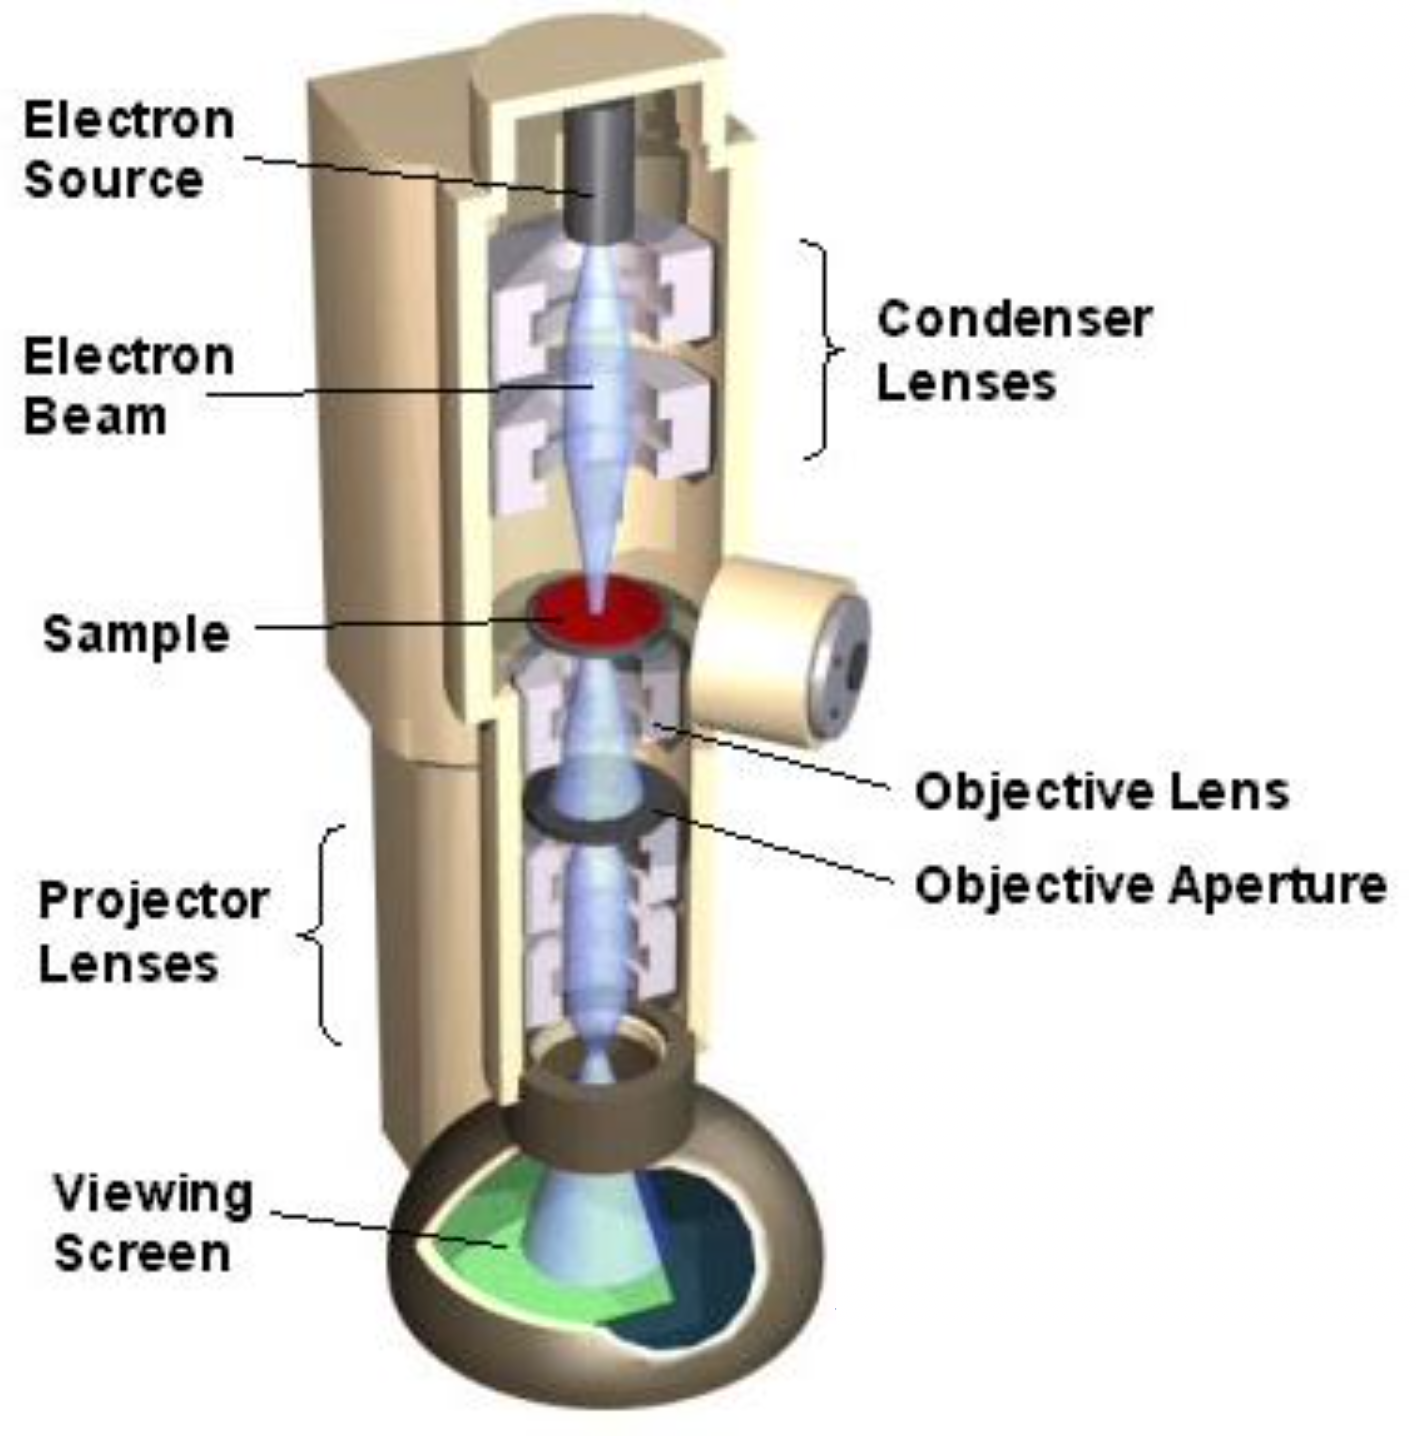
\includegraphics[width=0.8\linewidth]{TEMBuildingBlocksa.png}
            \caption{3D picture.}
            \label{fig:TEMBuildingBlocksa}
        \end{subfigure}
        \begin{subfigure}[b]{0.4\linewidth}
            \centering
            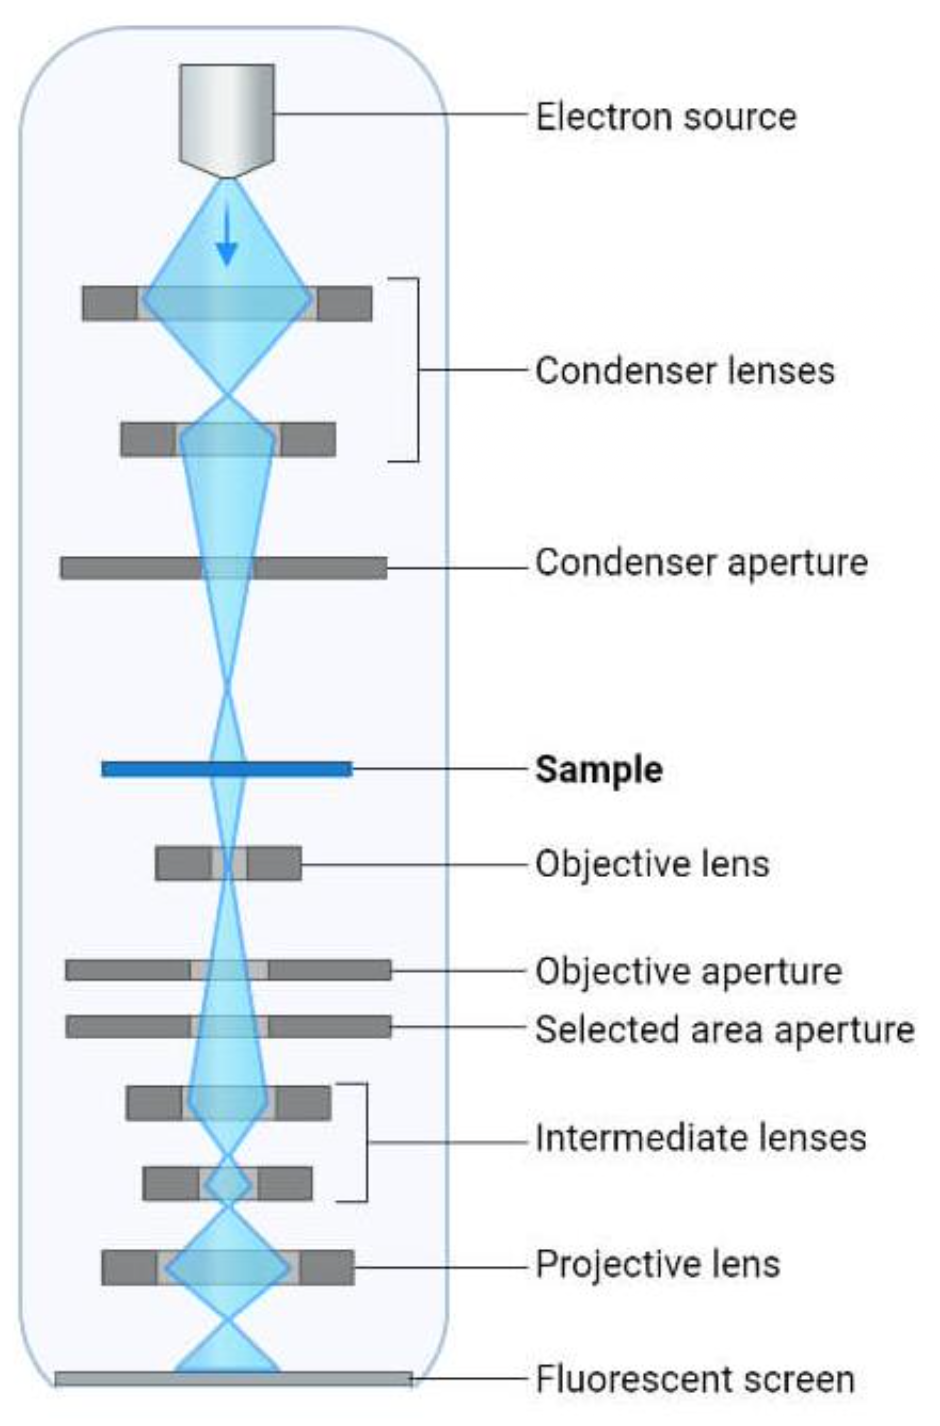
\includegraphics[width=0.55\linewidth]{TEMBuildingBlocksb.png}
            \caption{2D picture.}
            \label{fig:TEMBuildingBlocksb}
        \end{subfigure}
        \caption{TEM building blocks.}
        \label{fig:TEMBuildingBlocks}
    \end{figure}
    \begin{itemize}
        \item \textbf{Electron source}, \textbf{electron beam}, \textbf{condenser lenses}, \textbf{sample}, \textbf{objective lens}, \textbf{objective aperture}, \textbf{projector lenses}, \textbf{viewing screen}.
    \end{itemize}
    \pagebreak
    \item Electron source.
    \begin{figure}[H]
        \centering
        \begin{subfigure}[b]{0.4\linewidth}
            \centering
            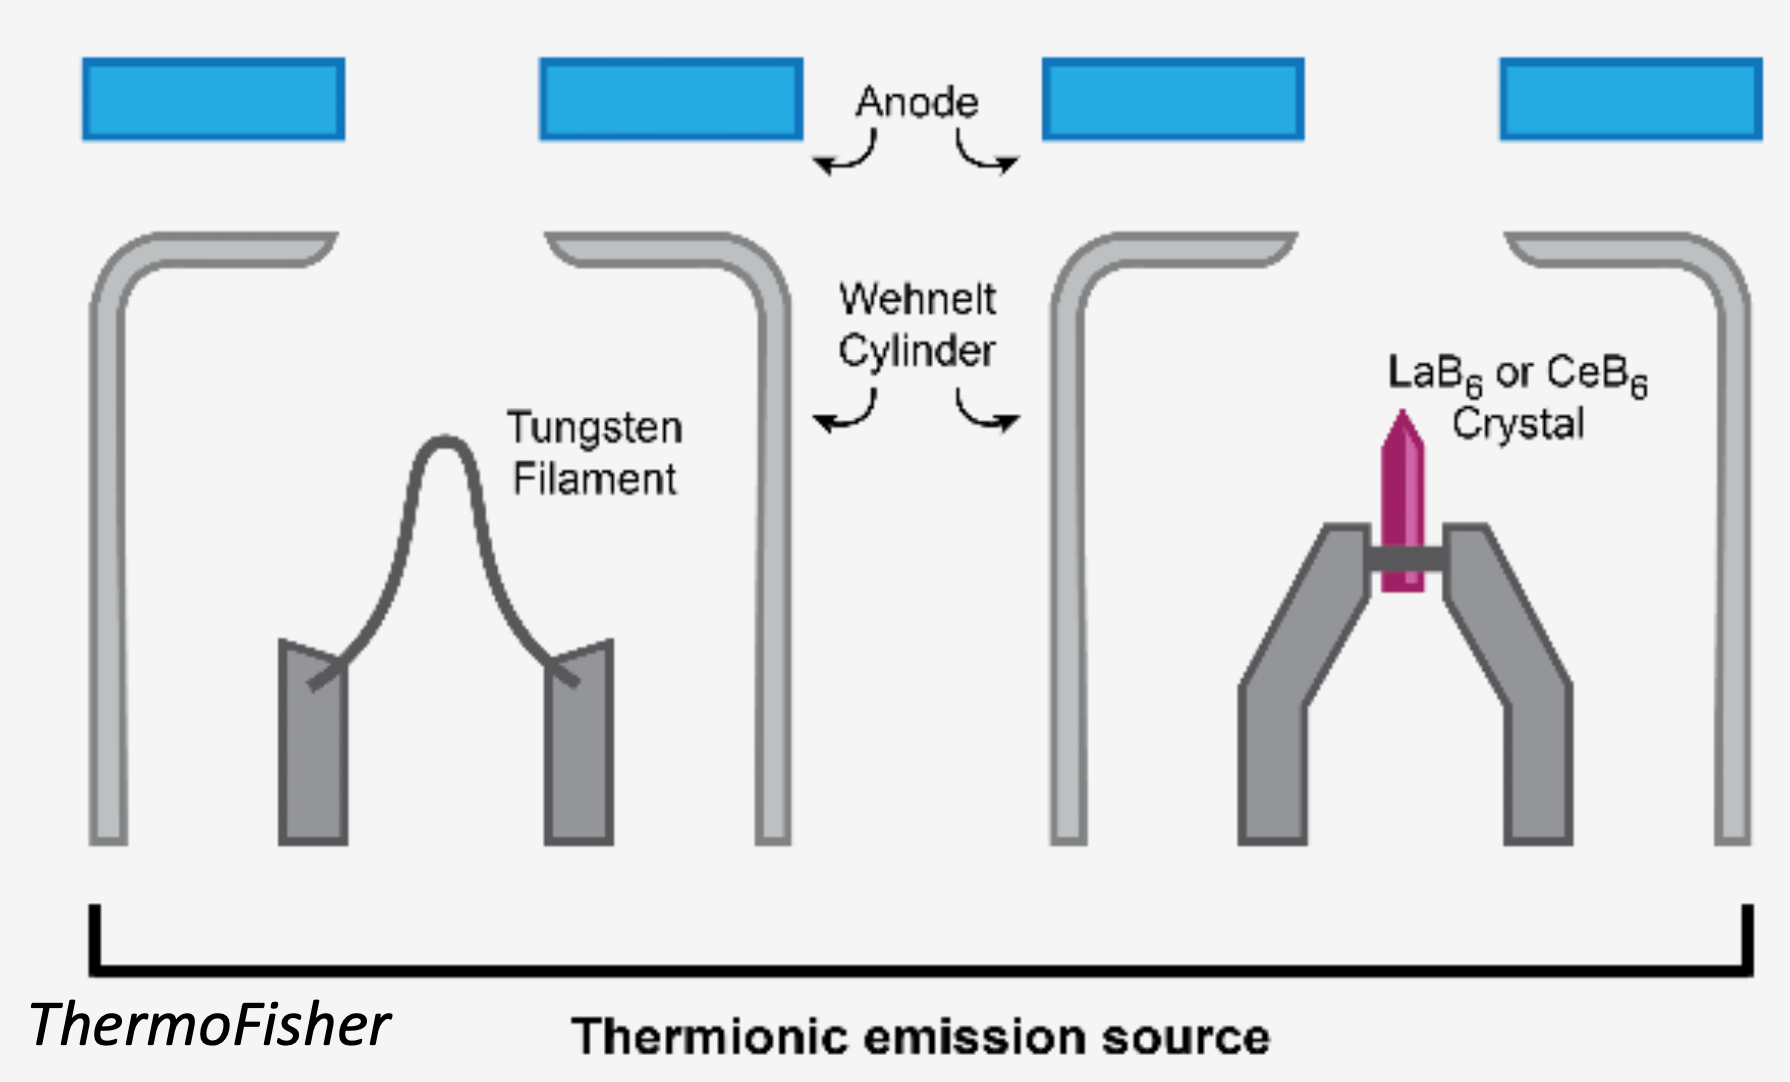
\includegraphics[width=0.9\linewidth]{TEMSourcea.png}
            \caption{Thermionic source.}
            \label{fig:TEMSourcea}
        \end{subfigure}
        \begin{subfigure}[b]{0.4\linewidth}
            \centering
            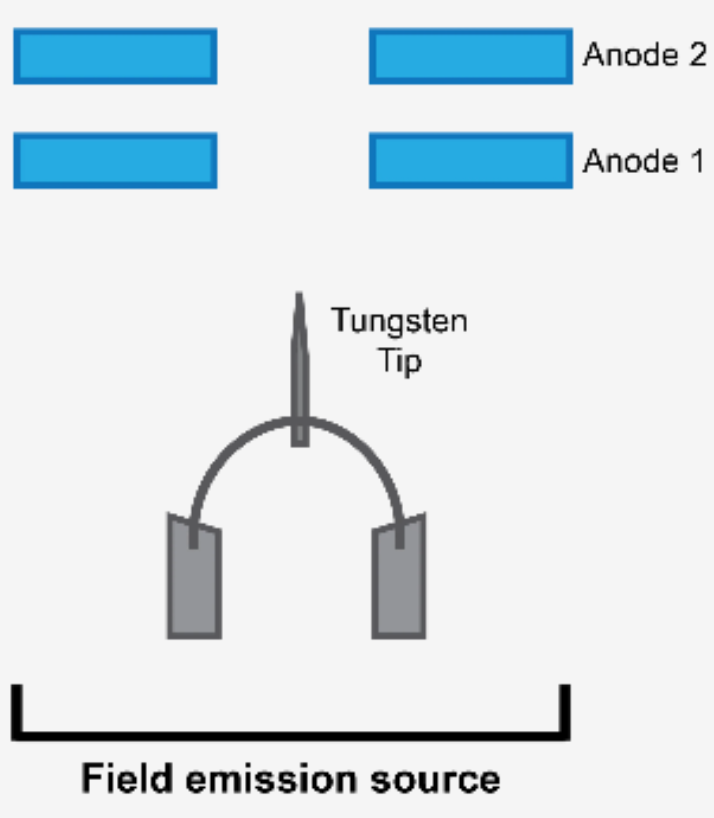
\includegraphics[width=0.45\linewidth]{TEMSourceb.png}
            \caption{Field Emission Gun.}
            \label{fig:TEMSourceb}
        \end{subfigure}
        \caption{TEM electron sources.}
        \label{fig:TEMSource}
    \end{figure}
    \begin{itemize}
        \item \textbf{Thermionic source} and \textbf{field emission gun}.
        \item A high voltage ($\sim\SIrange{60}{300}{\kilo\volt}$) is applied.
    \end{itemize}
    \item \textbf{Thermionic emission}: Emission of electrons into a vacuum achieved by applying a current (e.g., to single crystal of \ce{LaB6}, \ce{CeB6}, or \ce{W}) and heating.
    \begin{itemize}
        \item \ce{W} is cheap and easy to replace, but evaporates and breaks; lower brightness, broad beam, and hence reduced image resolution.
        \item \ce{LaB6} and \ce{CeB6}: Lower temperatures, lower beam spread, higher brightness, less volatile than tungsten (longer life time). But requires a higher vacuum (more expensive).
    \end{itemize}
    \item \textbf{Field Emission Gun}: A strong electrostatic field is applied to a sharply pointed tip of \ce{W}, leading to the release of high-energy electrons. \emph{Also known as} \textbf{FEG}.
    \begin{itemize}
        \item Developed by Albert Victor Crewe and Hittachi (1964 at UChicago).
        \item The emission area is small and hence brightness is high; enhanced image quality (high spatial resolution and increased signal-to-noise ratio); last long; but expensive (require very high vacuum).
    \end{itemize}
    \item \textbf{Schottky FEG}: A FEG that combines the thermionic and FEG sources (\ce{W} coated with \ce{ZrO2}).
    \item \textbf{Cold FEG}: Another type of FEG. \emph{Also known as} \textbf{CFEG}.
    \begin{itemize}
        \item Schottky FEGs have shorter lifetimes than CFEGs and worse image quality because of a larger energy spread, but better stability.
    \end{itemize}
    \item Relativistic and non-relativistic electron KE vs. wavelength curves.
    \begin{itemize}
        \item Also data on the accelerating voltage vs. frequency and wavelength.
        \item Significance??
    \end{itemize}
    \item Voltage: $\lambda$ correlations.
    \begin{itemize}
        \item Electrons are accelerated by the applied voltage $V$ and thus gain kinetic energy $mv^2/2$ (or, equivalently, $eV$ where $e$ is the charge of the electron).
        \item Since $\lambda_B=h/mv$, increasing $v=(eV/m)^{1/2}$ decreases the wavelength.
        \item Combining these two equations and plugging in values for $h,m,e$, we learn that
        \begin{equation*}
            \lambda_B = \frac{h}{(2meV)^{1/2}}
            = \frac{12.3}{V^{1/2}}
        \end{equation*}
        \item The $A$??
    \end{itemize}
    \item \textbf{Condenser lens}: An electromagnetic or electrostatic lens that is used in an electron microscope to guide and focus the electrons.
    \begin{itemize}
        \item The first lens through which the electrons pass (C1) determines the \textbf{spot size}.
        \item The second lens through which the electrons pass (C2) varies the \textbf{brightness}.
    \end{itemize}
    \item \textbf{Spot size}: The illumination spot on the sample.
    \item \textbf{Brightness}: The amount of illumination of the specimen.
    \item Aperture.
    \begin{itemize}
        \item The origin of spherical aberration.
        \begin{itemize}
            \item Electrons pass through the lens.
            \item Those at the periphery of the lens are refracted more than those in the middle.
            \item All the electrons will therefore not reach a common focal point.
        \end{itemize}
        \item Solution: An aperture is used to eliminate some of the peripheral electrons.
        \item The aperture also helps control the amount of illumination reaching the specimen.
        \item The origin of chromatic aberration.
        \begin{itemize}
            \item High energy electrons get deflected more??
            \item Ask more about this??
        \end{itemize}
    \end{itemize}
    \item Specimen area.
    \begin{figure}[h!]
        \centering
        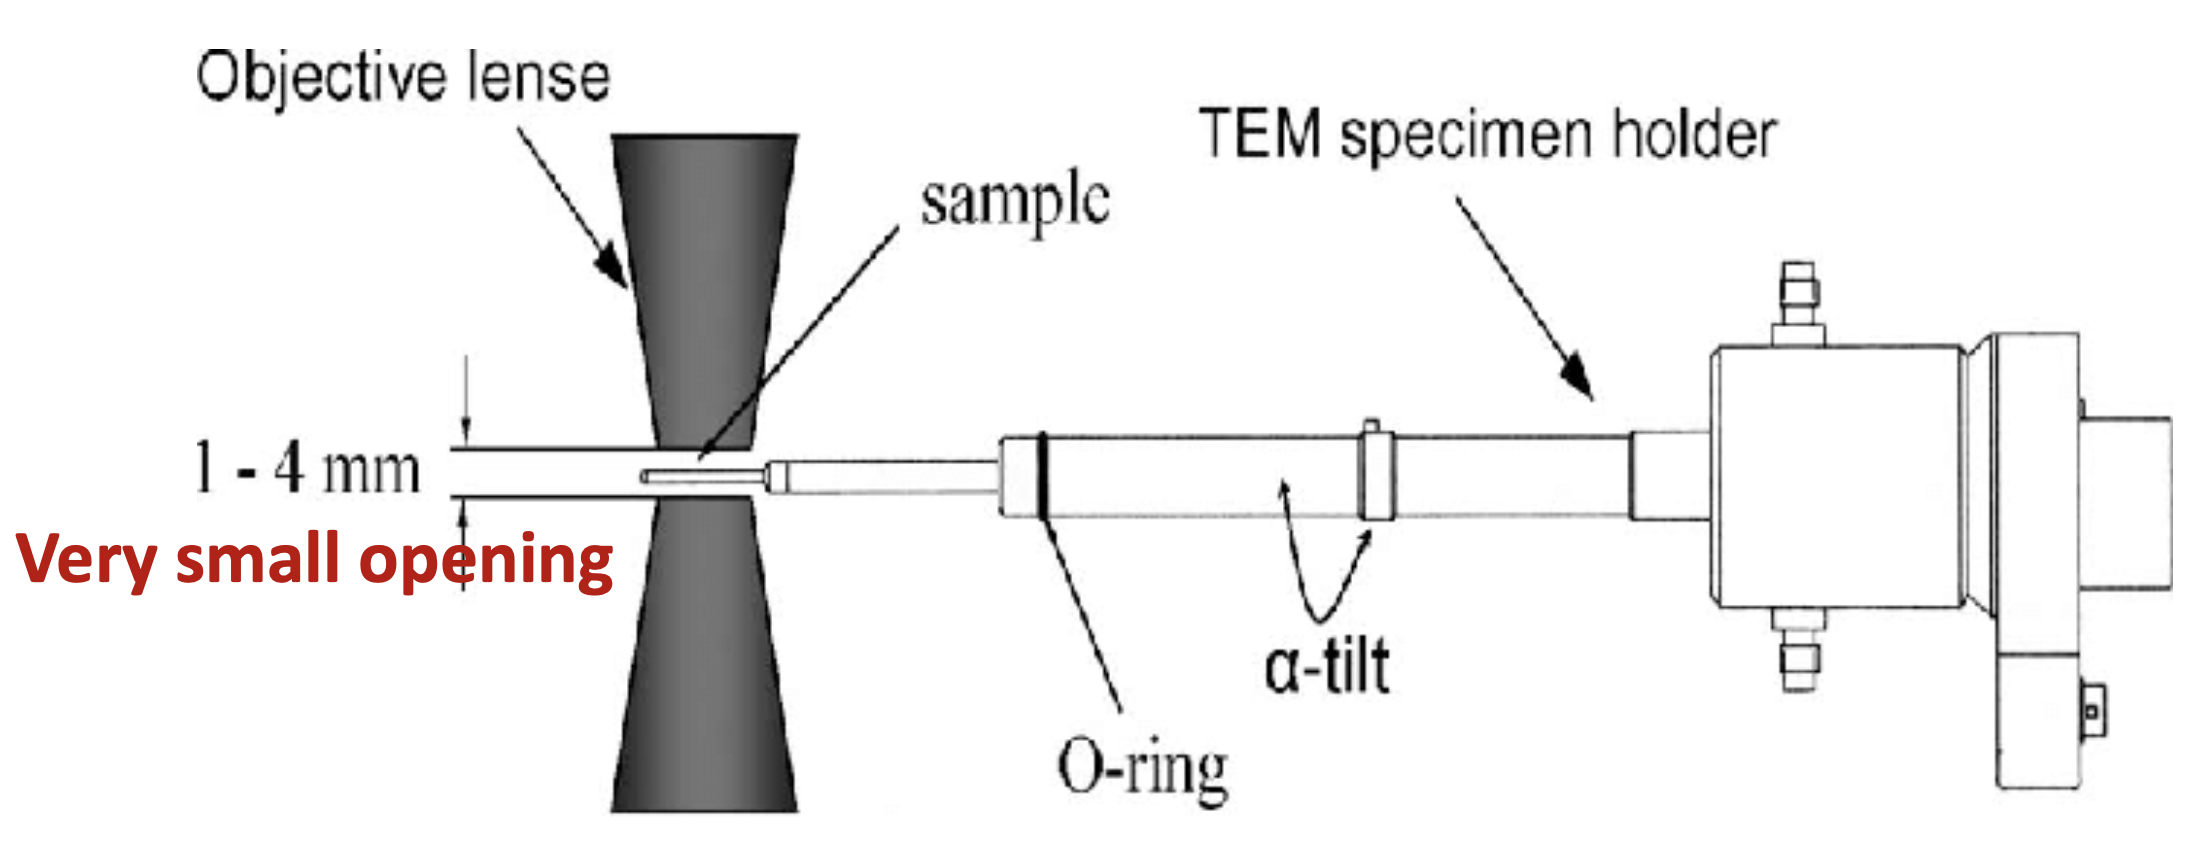
\includegraphics[width=0.6\linewidth]{TEMSampleHolder.png}
        \caption{Sample holder for TEM.}
        \label{fig:TEMSampleHolder}
    \end{figure}
    \begin{itemize}
        \item The sample is inserted using a sample holder.
        \begin{itemize}
            \item Sample holders come in many shapes and sizes. There are regular \textbf{JEOLs}, JEOL high tilt retainers, multiple sample models, etc.
            \item They can be further specialized for sample rotation (single tilt, double tilt, etc.), sample heating, or \emph{in situ} experiments.
        \end{itemize}
        \item The basic design is a long arm that extends to a gap between the objective lenses.
    \end{itemize}
    \item Objective lenses.
    \begin{itemize}
        \item \textbf{Objective lenses} and \textbf{objective apertures}.
    \end{itemize}
    \item \textbf{Objective lens}: A lens that forms, magnifies, and focuses the first image. \emph{Also known as} \textbf{OL}.
    \item \textbf{Objective aperture}: A lens that cuts off peripheral electrons to control contrast and spherical aberration. \emph{Also known as} \textbf{OA}.
    \begin{itemize}
        \item The OA consists of two \textbf{polepieces}, an upper and a lower one, surrounding the specimen holder from above and below. They are oppositely charged and create an appropriate field.
    \end{itemize}
    \item Intermediate lenses.
    \begin{itemize}
        \item These magnify the image from the OL and focus the diffraction pattern.
        \item There is also an \textbf{intermediate aperture} that is a diffraction aperture responsible for choosing the diffracted area.
    \end{itemize}
    \item Projective lenses.
    \begin{itemize}
        \item Magnify the image/control magnification.
    \end{itemize}
    \item Imaging systems.
    \begin{itemize}
        \item A fluorescent screen or a \textbf{CCD} (\textbf{charge coupled device}) camera.
        \item The CCD records in a digital format.
    \end{itemize}
    \item Astigmation.
    \begin{itemize}
        \item Reviews astigmation (see Figure \ref{fig:astigmation} and the above discussion).
        \item Stigmators are located in the condenser and objective lenses.
    \end{itemize}
    \item Origin of image contrast in TEM.
    \begin{itemize}
        \item Mass contrast: Absorption differences for different materials.
        \begin{itemize}
            \item Dark contrast refers to the heavy element/large atom number/thick sample.
            \item In other words, the darker regions of the image depict thicker or heavier samples.
        \end{itemize}
        \item Diffraction contrast: Contrast depends critically on diffraction conditions.
        \item Phase contrast: Contrast that depends on the phase shift of electrons passing through the sample.
        \begin{itemize}
            \item Lorentz microscopy and electron holography.
        \end{itemize}
        \item High-angle annular dark field (HAADF) imaging.
        \begin{itemize}
            \item Also known as scanning TEM (STEM) contrast.
            \item A function of atomic number.
        \end{itemize}
    \end{itemize}
    \item Mass contrast.
    \begin{itemize}
        \item Same as above.
    \end{itemize}
    \item Sample preparation.
    \begin{itemize}
        \item We use special TEM grids.
        \item There is often some polishing involved, also with polishing paper.
        \item \textbf{Ion milling} can be used.
    \end{itemize}
    \item \textbf{Ion milling}: Removal of the top layer of atoms.
    \begin{itemize}
        \item A \ce{Ga} ion source is often used.
        \item This is composed of \ce{Ga} in contact with a sharp \ce{W} tip.
        \item The electric field induces ionization and field emission of \ce{Ga+}.
        \item Focusing is done by an electrostatic lens.
    \end{itemize}
    \item Typical TEM images of nanoparticles and nanowires.
    \begin{itemize}
        \item Many examples shown, including \ce{CdSe}, \ce{CdS}, \ce{Fe_xO_y}, etc.
    \end{itemize}
    \item \ce{Ag}/\ce{AgCl} dimer.
    \begin{itemize}
        \item Mass contrast differentiates \ce{Ag} and \ce{AgCl}.
    \end{itemize}
    \item Structural rearrangements in \ce{Au} nanoparticles at high temperatures.
    \begin{itemize}
        \item Beam heating, laser heating, and thermal heating (i.e., in a small furnace holder) can all be used to observe phase changes, structural changes, etc.
    \end{itemize}
    \item TEM images of carbon nanomaterials.
    \begin{itemize}
        \item Several examples.
    \end{itemize}
    \item Dislocation upon nucleation (2D-to-3D transition).
    \begin{itemize}
        \item Strained 2D layers become strain-free 3D islands.
        \item Significance??
    \end{itemize}
    \item Electronic devices with nanoparticle superstructures.
    \begin{itemize}
        \item Pictures of computer-y stuff.
    \end{itemize}
    \item More nanoparticle pictures.
    \begin{itemize}
        \item Significance??
    \end{itemize}
\end{itemize}




\end{document}